\chapter[Introdução]{Introdução}
\label{cap:intro}

A Internet das Coisas, mais conhecida pelo seu acrônimo em inglês IoT (\emph{Internet of Things}), foi cunhada pelo engenheiro britânico Kevin Ashton no final dos anos 1990 onde ele, trabalhando para a empresa multinacional P\&G (Procter \& Gamble), pensou na possibilidade de que os produtos da empresa estivessem munidos de identificadores e capazes de estabelecer comunicação através da Internet, que na época estava se estabelecendo, criando assim uma rede em que as coisas estivessem conectadas \cite{KA_IOT}. Assim, os computadores se tornariam capazes de rastrear e identificar tudo, podendo reduzir desperdícios, minimizar custos e identificar o momento certo quando substituir ou reparar um produto \cite{lopezIOT}.

IoT, como a interconexão de dispositivos, representada na Figura \ref{fig:iot}, vem ganhado força ao longo dos anos, graças ao estudo, prototipação e desenvolvimento de diversos protocolos e tecnologias. Os pontos chave para o seu desenvolvimento foram a miniaturização de processadores e sensores; melhoramento e otimização do uso de baterias; definição de novos protocolos de rede e aumento da robustez de protocolos de comunicação sem fio.

\begin{figure}[ht]
      \begin{center}
            \caption{RSSF - Topologia Estrela}
            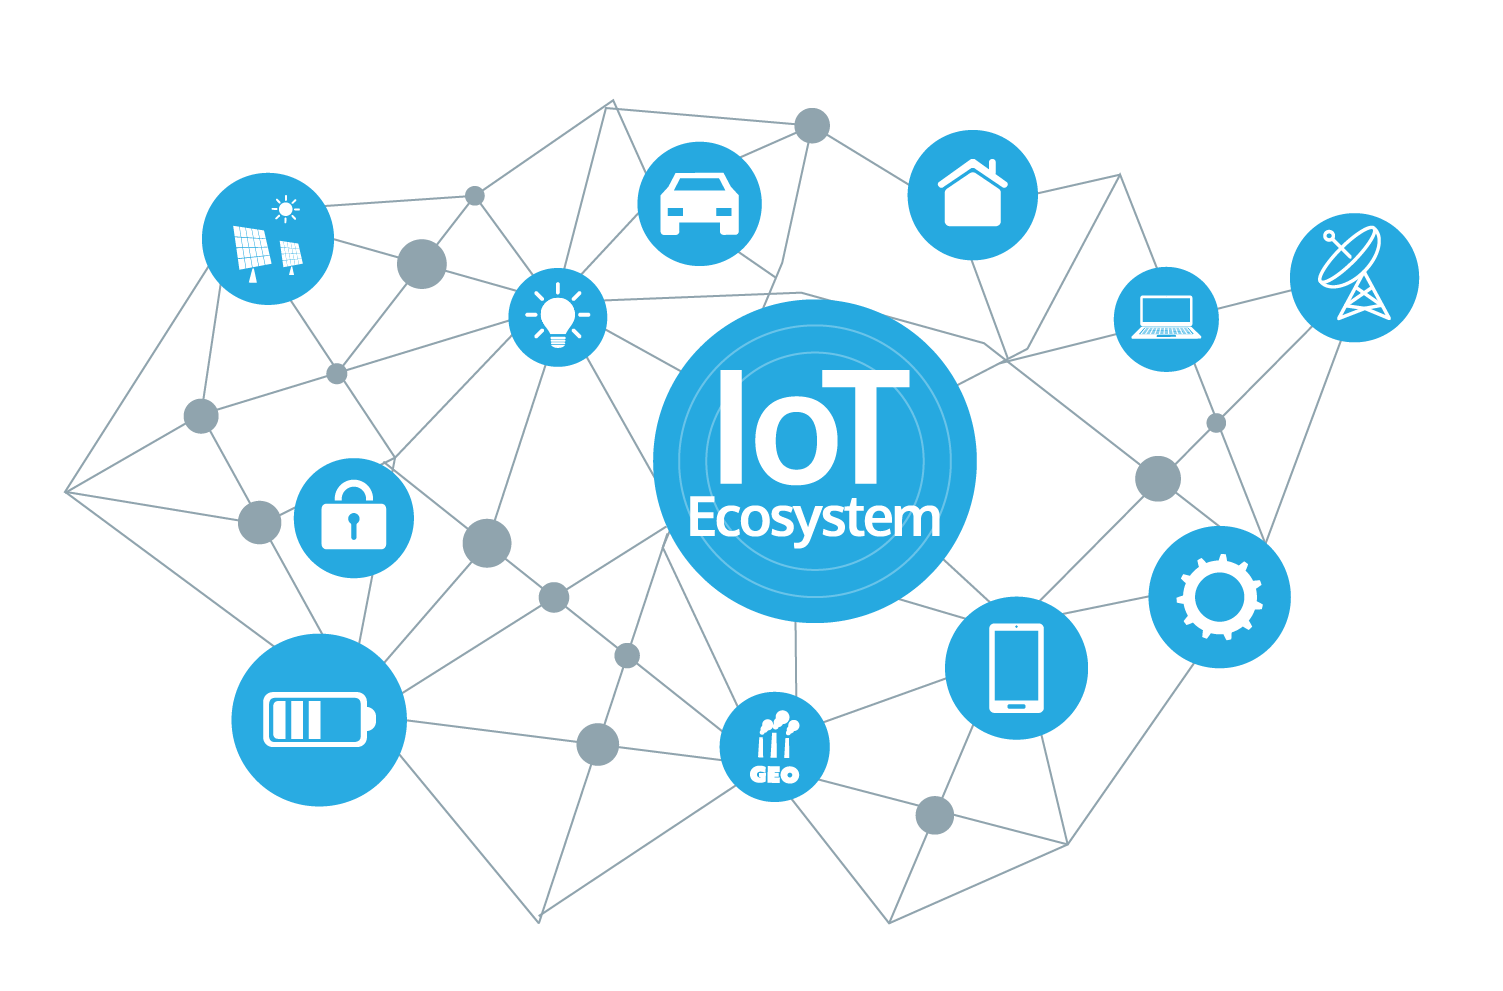
\includegraphics[width=10cm]{./sections/textual/chapters/images/iot.png}\\
            Fonte: copiada de \cite{figIoT}
            \label{fig:iot}
      \end{center}
\end{figure}

Atualmente há diversas aplicações de IoT, há implementações em larga escala como cidades inteligentes conforme descrito em \cite{sotres2017practical}, como em Santander na Espanha onde foram implementados por toda a cidade diversos nós com múltiplos sensores, afim de disponibilizar uma plataforma de testes. Há também aplicações de \emph{smart campus} como a apresentada em \cite{wang2017performance} com uma rede de sensores sem fio para verificar a qualidade do ar. Há aplicações de saúde como em \cite{zhang2015remote}, com coleta e análise em tempo real de informações de pressão sanguínea e massa corporal do paciente, para verificar a probabilidade do paciente ter um evento de insuficiência cardíaca, utilizando técnicas de aprendizado de máquina.

% Após o termo ser cunhado em 1999, foram necessários anos de evolução tecnológica para a atual popularidade do conceito. Por exemplo, a criação da plataforma de desenvolvimento de hardware aberta Arduino em 2005 \cite{OC_ARDUINO}, tornou fácil o estudo e a prototipação de itens de baixo custo. \ff{adicionar exemplos como o IPv6, baterias e os protocolos de Sem Fio}

A implementação de uma aplicação IoT necessita de uma rede de nós sensores distribuídos, geralmente conectados a um nó central, conhecido como nó \emph{gateway}, que tem por finalidade encaminhar os dados coletados para processamento. Para tal implementação existe duas abordagens clássicas: conexões cabeadas entre os nós da rede e a utilização de redes sem fio \cite{gomes2017estimaccao}. Como vantagem em relação às redes sem fio, as conexões cabeadas apresentam maior confiabilidade na conexão. Em contrapartida, a utilização de redes sem fio se destaca, em relação às redes cabeadas, nos quesitos de flexibilidade, custo de implantação, facilidade e rapidez na implementação e na manutenção \cite{gungor2009industrial}.

As Redes de Sensores Sem Fio (RSSF) se destacam na implementação de aplicações IoT, porém, há desafios para uma implementação robusta de comunicações sem fio, pois o meio de transmissão é caótico e pouco confiável. Interferências, ruídos, sombreamento e propagação por múltiplos percursos no meio podem ocasionar altas taxas de perda de pacotes e alta latência \cite{gomes2017estimaccao}.

Para contornar os desafios da comunicação sem fio, padrões e tecnologias foram desenvolvidos. Um dos principais órgãos na padronização em telecomunicações é o Instituto de Engenheiros Eletricistas e Eletrônicos, \emph{Institute of Electrical and Electronics Engineers}, mais conhecido pela sigla IEEE. Por exemplo, para redes locais, o Wi-Fi, baseado no padrão IEEE 802.11, se tornou uma tecnologia confiável que pode apresentar altas taxas de transmissão com baixa latência. Em redes de curto alcance, o Bluetooth, baseado no padrão IEEE 802.15.1, se tornou comum na vida das pessoas com seu uso para conexão de fones de ouvido, teclados e mouses sem fio. Estes padrões, apesar de bem estabelecidos no mercado, possuem alguns problemas para o desenvolvimento de RSSF, que geralmente requerem múltiplos dispositivos espalhados e, principalmente, sem acesso fácil a uma fonte contínua de energia.

Tendo em vista este problema energético, alguns padrões foram desenvolvidos para oferecer uma comunicação de qualidade, focando em eficiência energética para a utilização de baterias. Iniciativas privadas desenvolveram, por exemplo, o SigFox\footnote{https://www.sigfox.com/en} e LoRa\footnote{https://lora-alliance.org/}. O IEEE desenvolveu o padrão 802.15.4 e o aprimorou ao longo dos anos com adição de emendas, que foram responsáveis pelo desenvolvimento de aplicações como ZigBee\footnote{https://zigbeealliance.org/} e Wi-SUN\footnote{https://wi-sun.org/}. A \emph{3rd Generation Partnership Project} (3GPP)\footnote{https://www.3gpp.org/} Projeto de Parceria de Terceira Geração em tradução livre, desenvolveu a tecnologia NB-IoT, uma versão simplificada da tecnologia de comunicação celular LTE,\emph{Longe Term Evolution} (Evolução de Longo Prazo), que visa utilizar a mesma infraestrutura, porém com melhor eficiência energética. Estas tecnologias podem ser utilizadas para a implementação de redes classificadas como Redes de Longo Alcance e Baixo Consumo Energético.

\section{Justificativa e Relevância do Trabalho}
\label{sec:justificativa}
Em \cite{tuset2020dataset}, os autores implementaram uma RSSF utilizando as modulações propostas na emenda ``g'' do padrão IEEE 802.15.4. O experimento foi realizado em um cenário industrial, durando 99 dias e gerou um conjunto de dados que foi utilizado para averiguar a confiabilidade da rede e, nesse caso, propor mecanismos de diversidade de modulação que, como mostrado em \cite{gomes2020improving}, podem melhorar a taxa de entrega de pacotes.

O cenário industrial apresenta diversos problemas, principalmente relacionados à interferência e propagação por múltiplos caminhos. Diferentes ambientes possuem diferentes problemas em relação a comunicação via rádio. Então, este trabalho tem como objetivo analisar a comunicação sem fio de transceptores do padrão IEEE 802.15.4g SUN em um ambiente predial, também denominado neste texto como \emph{Smart Building}, cuja principal fonte de problemas para a comunicação é a falta de linha de visada. Devem ser estudadas as características da RSSF a partir da verificação da taxa de entrega de pacotes e verificar sua viabilidade de implementação com a tecnologia utilizada.

\section{Objetivos}
\label{sec:objetivos}

\subsection{Objetivo Geral}
\label{subsec:objGeral}
Coletar e analisar as informações das transmissões de uma RSSF realizadas com as modulações definidas no padrão IEEE 802.15.4g em um cenário de \emph{smart building}.

% Coletar e analisar os dados experimentais de transmissões realizadas entre os dispositivos openmote que implementam as modulações definidas no padrão IEEE 802.15.4g SUN espalhados pelo prédio dos professores no campus Campina Grande.

\subsection{Objetivos Específicos}
\label{subsec:objespecificos}
\begin{itemize}
      \item Implementar uma RSSF utilizando transceptores que implementam as modulações do IEEE 802.15.4g;
      \item Coletar os dados das transmissões realizadas;
      \item Avaliar o desempenho da rede implementada, a partir da análise dos dados coletados.
\end{itemize}


\section{Metodologia}
\label{sec:metodologia}
Para alcançar tais objetivos, foram realizados os seguintes passos:

% Estudei a plataforma de desenvolvimento do Openmote
% Fiz as mudanças no código de Pere
% fiz o código python dos gateways/persistência dos dados no influx
% Colocar pra rodar o experimento
% analise dos dados

\begin{itemize}
      \item Estudo e implementação dos dispositivos: Entender o funcionamento dos dispositivos que utilizam o código-fonte presente em \cite{openmoteb-firmware}. E a realização de alterações no código-fonte para a aplicação proposta;
      \item Desenvolvimento do \emph{gateway}: Criar \emph{scripts} para utilização de um computador como gateway da rede, capaz de coletar os dados das transmissões e persisti-los em um banco de dados;
      \item Execução do experimento: Distribuir os nós transmissores pelo prédio, conectar os nós receptores ao gateway e coletar dados;
      \item Análise dos resultados: Com os dados gerados, realizar sua análises, que é apresentada no Capítulo \ref{resultados}.
\end{itemize}